\begin{figure}[H]\centering
  \begin{subfigure}{0.49\linewidth}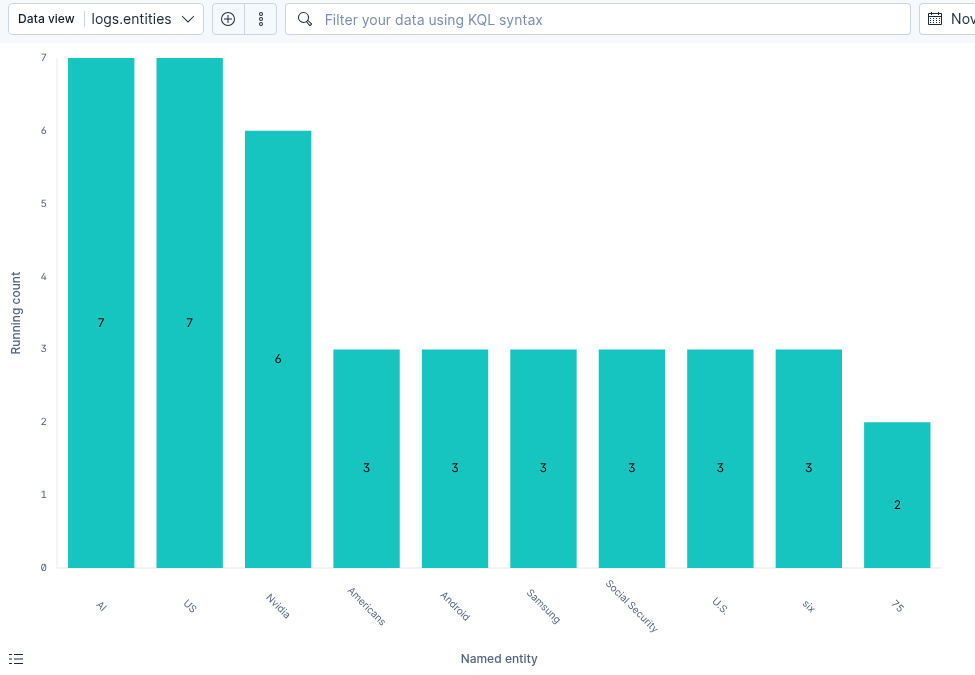
\includegraphics[width=\linewidth]{outputs/kibana_top10_15min.png}\caption{$t=15$
    min}
  \end{subfigure}\hfill
  \begin{subfigure}{0.49\linewidth}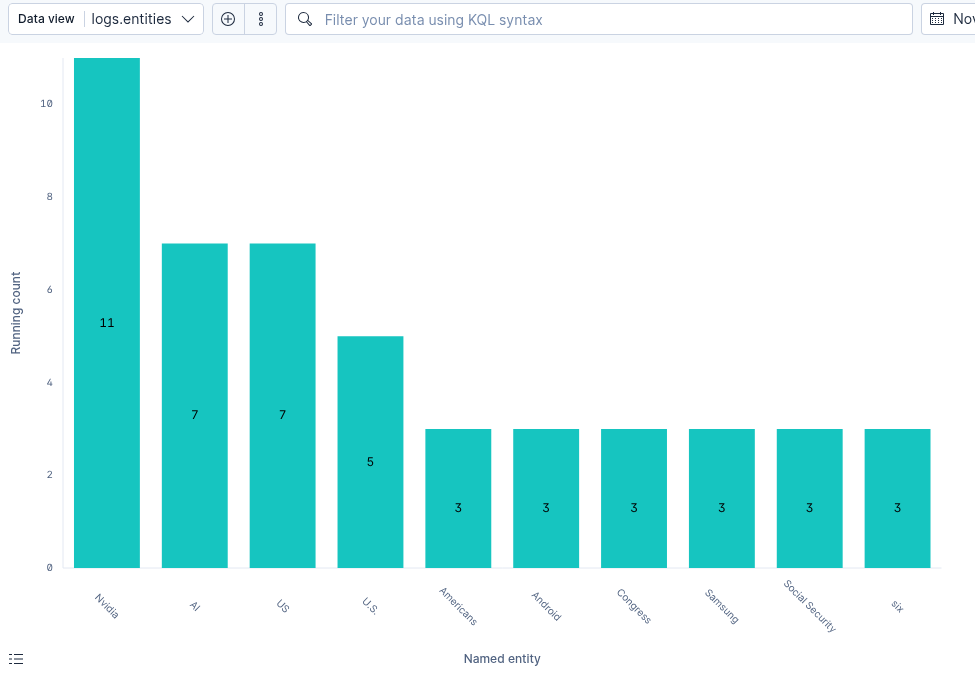
\includegraphics[width=\linewidth]{outputs/kibana_top10_30min.png}\caption{$t=30$
    min}
  \end{subfigure}

  \begin{subfigure}{0.49\linewidth}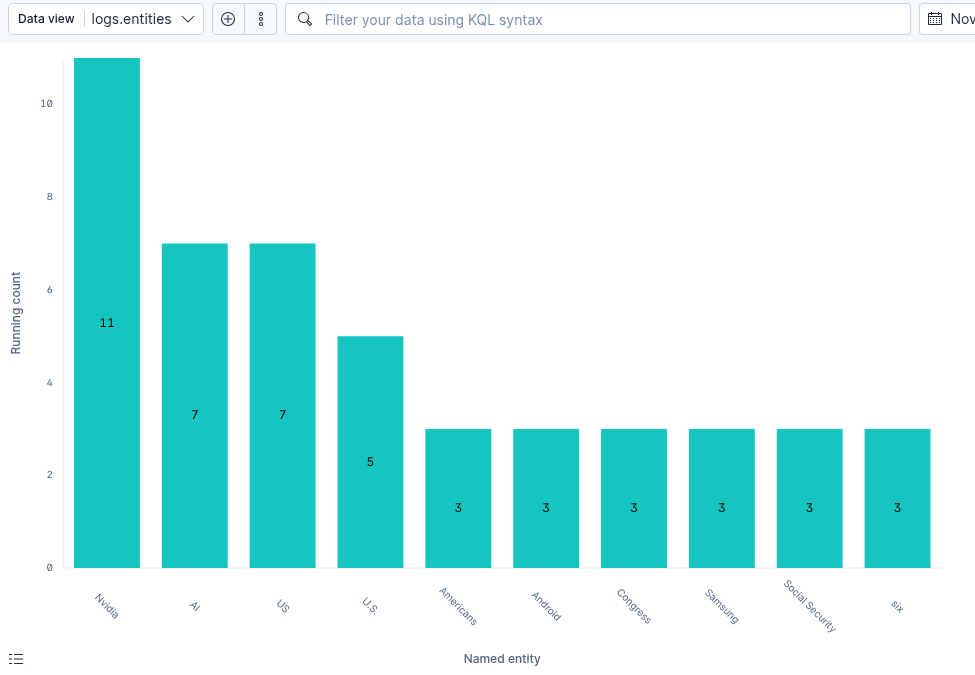
\includegraphics[width=\linewidth]{outputs/kibana_top10_45min.png}\caption{$t=45$
    min}
  \end{subfigure}\hfill
  \begin{subfigure}{0.49\linewidth}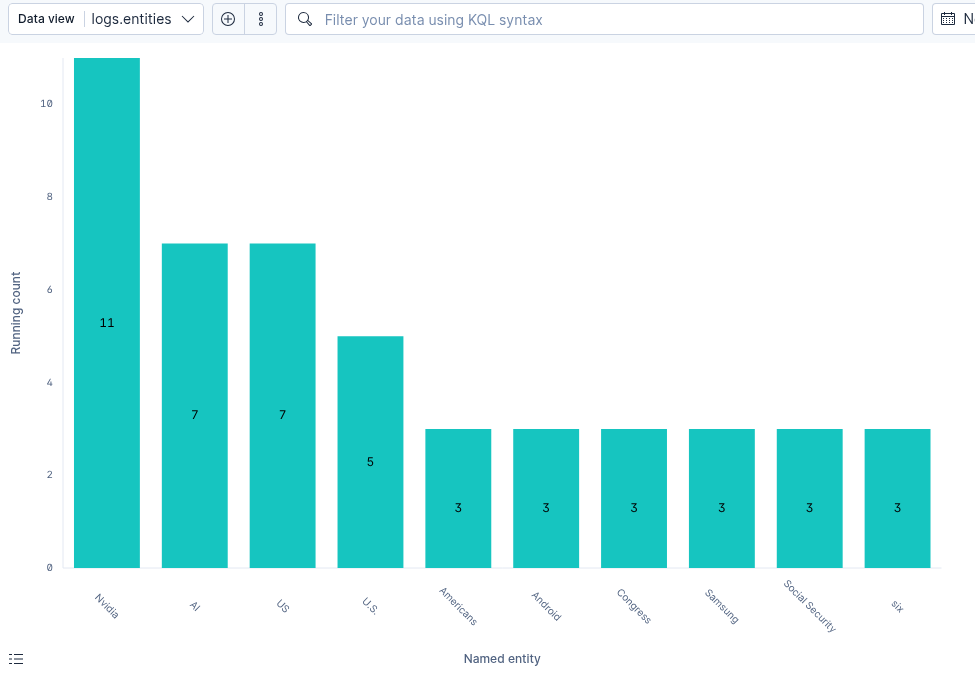
\includegraphics[width=\linewidth]{outputs/kibana_top10_60min.png}\caption{$t=60$
    min}
  \end{subfigure}
  \caption{Kibana bar plots of the top 10 named entities (running
  count) after 15, 30, 45 and 60 minutes.}
  \label{fig:kibana}
\end{figure}

\begin{table}[H]\centering\footnotesize\setlength{\tabcolsep}{3pt}
  \begin{subtable}[t]{0.45\linewidth}\centering\begin{tabular}{rlr}
\toprule
Rank & Entity & Count \\
\midrule
1 & AI & 7 \\
2 & US & 7 \\
3 & Nvidia & 6 \\
4 & Americans & 3 \\
5 & Android & 3 \\
6 & Samsung & 3 \\
7 & Social Security & 3 \\
8 & U.S. & 3 \\
9 & six & 3 \\
10 & 75 & 2 \\
\bottomrule
\end{tabular}
\caption{15
    min}\label{tab:ent15}
  \end{subtable}\hfill
  \begin{subtable}[t]{0.45\linewidth}\centering\begin{tabular}{rlr}
\toprule
Rank & Entity & Count \\
\midrule
1 & Nvidia & 11 \\
2 & AI & 7 \\
3 & US & 7 \\
4 & U.S. & 5 \\
5 & Americans & 3 \\
6 & Android & 3 \\
7 & Congress & 3 \\
8 & Samsung & 3 \\
9 & Social Security & 3 \\
10 & six & 3 \\
\bottomrule
\end{tabular}
\caption{30
    min}\label{tab:ent30}
  \end{subtable}

  \vspace{0.8em}
  \begin{subtable}[t]{0.45\linewidth}\centering\begin{tabular}{rlr}
\toprule
Rank & Entity & Count \\
\midrule
1 & Nvidia & 11 \\
2 & AI & 7 \\
3 & US & 7 \\
4 & U.S. & 5 \\
5 & Americans & 3 \\
6 & Android & 3 \\
7 & Congress & 3 \\
8 & Samsung & 3 \\
9 & Social Security & 3 \\
10 & six & 3 \\
\bottomrule
\end{tabular}
\caption{45
    min}\label{tab:ent45}
  \end{subtable}\hfill
  \begin{subtable}[t]{0.45\linewidth}\centering\begin{tabular}{rlr}
\toprule
Rank & Entity & Count \\
\midrule
1 & Nvidia & 11 \\
2 & AI & 7 \\
3 & US & 7 \\
4 & U.S. & 5 \\
5 & Americans & 3 \\
6 & Android & 3 \\
7 & Congress & 3 \\
8 & Samsung & 3 \\
9 & Social Security & 3 \\
10 & six & 3 \\
\bottomrule
\end{tabular}
\caption{60
    min}\label{tab:ent60}
  \end{subtable}
  \caption{Top-10 entities read from Elasticsearch at each capture
  (\texttt{outputs/entities\_*min.json}).}
\end{table}

\paragraph{Throughput.} The poller ran five times (00, 15, 30, 45 and 60 min).
The first poll published 19 headlines. The 15-minute poll returned only stories
already sent. The 30-minute poll (19:14) added 6 new headlines. The 45- and
60-minute polls again returned nothing new. Topic \texttt{articles} therefore
holds 25 articles, which produced 113 distinct entities. Spark only runs a
micro-batch when new input arrives, so \texttt{logs.entities} received two
batches (84 records at $t\approx0$, 113 at $t\approx30$\,min).

\paragraph{Reflections}

The named entity extraction via spaCy could have been handled more
carefully and more effeciently. Namely, normalising
aliases and keeping only \texttt{PERSON}, \texttt{ORG}, \texttt{GPE} and
\texttt{PRODUCT} labels would give a cleaner ranking. Further, the
current architecture which registers the spaCy extractor as a duf
loads the model on every call, and if we were to switch to a more
capable model that could become expensive, as a work around it is
possible to either serialize the model as a broadcast variable to
every worker node, or have it load only once on every node via some
local state.
